\section{Coffee in society}
\label{sec:coffee-in-society}
In recent years, coffee has gained more and more popularity, cementing itself as one of the most widely consumed beverages.
Along with a surge in café openings, preparing coffee at home is now an activity enjoyed by more and more people, with the average consumer being more discerning and critical than ever.

The development of the coffee industry is often described as a series of ``waves''.
The first ``wave'' made coffee an everyday staple, focusing on convenience and high availability.
During the second wave, the idea of ``specialty'' coffee first entered the consumer vocabulary, with creative recipes, flavours and textures being popularised by emerging cafés and chains.
The third wave, starting around 1980 and lasting to the present day saw a significant shift in consumer values:
rather than adding additional flavours in their coffee drinks, the consumers instead started noticing the taste characteristics of the beans themselves,
with simpler, more delicately flavoured drinks being preferred.
It is also during this time that coffee processing and roasting were moved into focus,
with the average consumer being more and more likely to differentiate and prefer a certain flavour profile over others.

The popularity of brewing ``specialty'' coffee at home has also risen during this time.
A coffee enthusiast is now more likely to own a grinder and one or more brewers, preferring to purchase whole-bean,
usually single-origin coffee, with the expectation of the resulting drink matching the advertised flavour and aroma notes.

It should also be noted that the preference in roast levels have also shifted as the waves changed.
During the second wave, when additional flavours and textures were the key focus of drinks,
a darker roast was preferred, as espresso produced with a darker roasted bean will have a more mellow,
sweet taste, with little to no acidity (though, a higher chance of bitterness if the coffee / water ratios are not correct),
and a thicker, heavier body.
With this style of preparation, an equal ratio of water to ground coffee is used, yielding a smaller, more intense espresso.

In contrast, a ``third-wave'' coffee preparation style values the acidity and floral notes that can only be retained
through a very light, gentle roasting process.
For many modern coffee enthusiasts, the lightest possible roast level is the most desirable.
While an under-roasted bean will taste unpleasant to a vast majority, with grassy, vegetal notes,
a roast level above ``medium'' is thought to mask away the harder to retain flavour notes
coming from either the coffee processing method, its origin or both.
As lighter roasted coffee is less soluble and therefore more difficult to extract,
modern coffee establishments often use higher coffee to water ratios, with 1:3 or even 1:5 ratios used to brew espresso.
Drinks brewed this way sacrifice a thicker body for clarity and brightness of flavour, exposing as much of the bean's
flavour profile as possible.
With the coffee flavour placed front-and-center, it is now more important than ever for coffee producers to deliver
the best possible quality of their product.

This shift of consumer patterns has placed a lot of importance on coffee roasters and farmers,
who are now held to a higher standard than ever before.
Even a small percentage of defects, whether in the green (unroasted) coffee or in the final product,
can ruin a brewed drink.
As environmental issues and quality control at farms is often out of the roasters' control,
it is therefore extremely important that the roasters are able to detect defects on their side
with as much precision as possible.


The following section will discuss the challenges faced by coffee roasters and producers
as well as describe the ``state of the art'' of quality control in coffee production.

\section{Coffee production challenges}\label{sec:coffee-production-challenges}
The worsening climate conditions, rising consumer expectations and economic instability are just a few of the challenges
faced by the coffee roasting industry.
As many roasteries are quite small businesses, addressing supply chain issues is often beyond their control,
with roasters having to perform secondary quality control to address the shortcomings of the previous stages in the beans'
journey.

Defective green coffee beans can seriously damage the flavour of the finished product.
The most common defect occurs when the coffee cherry does not develop the necessary sugar content
due to being harvested before fully maturing or disease of the plant:
the beans within these cherries do not respond well to roasting, developing an extremely unpleasant flavour
which is typically compared to burnt paper, with an astringent, drying sensation in the mouth.
Such beans are commonly referred to as ``quakers'' and, when roasted, can be identified by
an uneven, spotty exterior as seen on figure \ref{fig:quakerBeanExample}.
The spotty pattern develops due to the lack of sugar, preventing the bean from fully caramelising during roasting.
\begin{wrapfigure}{r}{0.5\textwidth}
    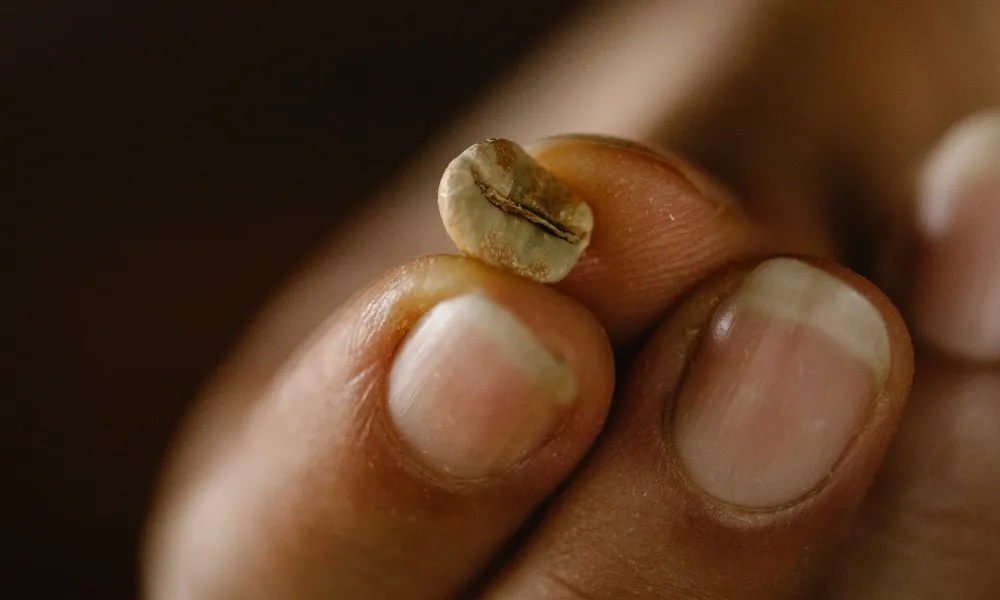
\includegraphics[width=0.5\textwidth]{quaker-coffee-bean}
    \caption*{Source: \cite{quakerBeanImg}}
    \caption{An example of a ``quaker'' coffee bean.}
    \label{fig:quakerBeanExample}
\end{wrapfigure}
The unpleasant flavour brought along by such beans is extremely potent, with just a few being able to ruin a large batch
of otherwise acceptable product.

Apart from harming the taste of the roasters' products, such beans can also prevent the roasters from achieving certain
certifications or using certain marketing language.
The Specialty Coffee Association (SCA) is one of the most influential regulatory bodies in the coffee industry.
The term ``specialty'' can only be used to describe coffee when certain criteria are achieved:
each batch of green coffee is roasted and tasted, with the tasters awarding points for various aspects of the drink's flavours.
In order to achieve specialty status, the coffee has to earn over 80 points, as well as being free from the previously mentioned defects.

As the ``specialty'' mark is often necessary for a roaster to stand out among its competition and make itself known to
coffee enthusiasts, quality control is one of the most important tasks that a coffee roaster faces on a daily basis.

\section{State of the art in coffee quality control}\label{sec:qc-state-of-the-art}
Despite the previously described importance of quality control, the automation options are surprisingly limited,
requiring many medium-to-small scale roasters to perform their quality control manually.
While the knowledge and expertise of many roasters allows them to perform this task relatively easily,
it still requires a significant amount of time and manual labour, preventing the roasters from performing other tasks.
Furthermore, this approach does not guarantee repeatable or even correct results,
depending fully on the judgement of the person performing it.

It should be noted that some commercial solutions are offered:
industrial scale colour graders can provide a high degree of accuracy and efficiency.
These machines use image recognition to place the beans in one of several pre-determined categories,
using blasts of compressed air to remove defective beans as they fall through the air.
\begin{wrapfigure}{r}{0.5\textwidth}
    \includegraphics[width=0.5\textwidth]{colour-sorter-scale}
    \caption*{Source: \cite{colourSorterImg}}
    \caption{A typical colour grader in a coffee roasting facility}
    \label{fig:colourSorterExample}
\end{wrapfigure}
These machines, however, are often a poor fit to all but the largest coffee roasters due to several reasons:
\begin{itemize}
    \item Prohibitive pricing
    \begin{itemize}
        \item Test
    \end{itemize}
    \item Large size
    \begin{itemize}
        \item Test
    \end{itemize}
    \item Unknown training dataset
    \begin{itemize}
        \item Test
    \end{itemize}
    \item Scale of production
    \begin{itemize}
        \item Test
    \end{itemize}
\end{itemize}


\section{Research aims}\label{sec:research-aims}